% Options for packages loaded elsewhere
% Options for packages loaded elsewhere
\PassOptionsToPackage{unicode}{hyperref}
\PassOptionsToPackage{hyphens}{url}
\PassOptionsToPackage{dvipsnames,svgnames,x11names}{xcolor}
%
\documentclass[
]{article}
\usepackage{xcolor}
\usepackage{amsmath,amssymb}
\setcounter{secnumdepth}{5}
\usepackage{iftex}
\ifPDFTeX
  \usepackage[T1]{fontenc}
  \usepackage[utf8]{inputenc}
  \usepackage{textcomp} % provide euro and other symbols
\else % if luatex or xetex
  \usepackage{unicode-math} % this also loads fontspec
  \defaultfontfeatures{Scale=MatchLowercase}
  \defaultfontfeatures[\rmfamily]{Ligatures=TeX,Scale=1}
\fi
\usepackage{lmodern}
\ifPDFTeX\else
  % xetex/luatex font selection
\fi
% Use upquote if available, for straight quotes in verbatim environments
\IfFileExists{upquote.sty}{\usepackage{upquote}}{}
\IfFileExists{microtype.sty}{% use microtype if available
  \usepackage[]{microtype}
  \UseMicrotypeSet[protrusion]{basicmath} % disable protrusion for tt fonts
}{}
\makeatletter
\@ifundefined{KOMAClassName}{% if non-KOMA class
  \IfFileExists{parskip.sty}{%
    \usepackage{parskip}
  }{% else
    \setlength{\parindent}{0pt}
    \setlength{\parskip}{6pt plus 2pt minus 1pt}}
}{% if KOMA class
  \KOMAoptions{parskip=half}}
\makeatother
% Make \paragraph and \subparagraph free-standing
\makeatletter
\ifx\paragraph\undefined\else
  \let\oldparagraph\paragraph
  \renewcommand{\paragraph}{
    \@ifstar
      \xxxParagraphStar
      \xxxParagraphNoStar
  }
  \newcommand{\xxxParagraphStar}[1]{\oldparagraph*{#1}\mbox{}}
  \newcommand{\xxxParagraphNoStar}[1]{\oldparagraph{#1}\mbox{}}
\fi
\ifx\subparagraph\undefined\else
  \let\oldsubparagraph\subparagraph
  \renewcommand{\subparagraph}{
    \@ifstar
      \xxxSubParagraphStar
      \xxxSubParagraphNoStar
  }
  \newcommand{\xxxSubParagraphStar}[1]{\oldsubparagraph*{#1}\mbox{}}
  \newcommand{\xxxSubParagraphNoStar}[1]{\oldsubparagraph{#1}\mbox{}}
\fi
\makeatother


\usepackage{longtable,booktabs,array}
\usepackage{calc} % for calculating minipage widths
% Correct order of tables after \paragraph or \subparagraph
\usepackage{etoolbox}
\makeatletter
\patchcmd\longtable{\par}{\if@noskipsec\mbox{}\fi\par}{}{}
\makeatother
% Allow footnotes in longtable head/foot
\IfFileExists{footnotehyper.sty}{\usepackage{footnotehyper}}{\usepackage{footnote}}
\makesavenoteenv{longtable}
\usepackage{graphicx}
\makeatletter
\newsavebox\pandoc@box
\newcommand*\pandocbounded[1]{% scales image to fit in text height/width
  \sbox\pandoc@box{#1}%
  \Gscale@div\@tempa{\textheight}{\dimexpr\ht\pandoc@box+\dp\pandoc@box\relax}%
  \Gscale@div\@tempb{\linewidth}{\wd\pandoc@box}%
  \ifdim\@tempb\p@<\@tempa\p@\let\@tempa\@tempb\fi% select the smaller of both
  \ifdim\@tempa\p@<\p@\scalebox{\@tempa}{\usebox\pandoc@box}%
  \else\usebox{\pandoc@box}%
  \fi%
}
% Set default figure placement to htbp
\def\fps@figure{htbp}
\makeatother


% definitions for citeproc citations
\NewDocumentCommand\citeproctext{}{}
\NewDocumentCommand\citeproc{mm}{%
  \begingroup\def\citeproctext{#2}\cite{#1}\endgroup}
\makeatletter
 % allow citations to break across lines
 \let\@cite@ofmt\@firstofone
 % avoid brackets around text for \cite:
 \def\@biblabel#1{}
 \def\@cite#1#2{{#1\if@tempswa , #2\fi}}
\makeatother
\newlength{\cslhangindent}
\setlength{\cslhangindent}{1.5em}
\newlength{\csllabelwidth}
\setlength{\csllabelwidth}{3em}
\newenvironment{CSLReferences}[2] % #1 hanging-indent, #2 entry-spacing
 {\begin{list}{}{%
  \setlength{\itemindent}{0pt}
  \setlength{\leftmargin}{0pt}
  \setlength{\parsep}{0pt}
  % turn on hanging indent if param 1 is 1
  \ifodd #1
   \setlength{\leftmargin}{\cslhangindent}
   \setlength{\itemindent}{-1\cslhangindent}
  \fi
  % set entry spacing
  \setlength{\itemsep}{#2\baselineskip}}}
 {\end{list}}
\usepackage{calc}
\newcommand{\CSLBlock}[1]{\hfill\break\parbox[t]{\linewidth}{\strut\ignorespaces#1\strut}}
\newcommand{\CSLLeftMargin}[1]{\parbox[t]{\csllabelwidth}{\strut#1\strut}}
\newcommand{\CSLRightInline}[1]{\parbox[t]{\linewidth - \csllabelwidth}{\strut#1\strut}}
\newcommand{\CSLIndent}[1]{\hspace{\cslhangindent}#1}



\setlength{\emergencystretch}{3em} % prevent overfull lines

\providecommand{\tightlist}{%
  \setlength{\itemsep}{0pt}\setlength{\parskip}{0pt}}



 


\makeatletter
\@ifpackageloaded{caption}{}{\usepackage{caption}}
\AtBeginDocument{%
\ifdefined\contentsname
  \renewcommand*\contentsname{Table of contents}
\else
  \newcommand\contentsname{Table of contents}
\fi
\ifdefined\listfigurename
  \renewcommand*\listfigurename{List of Figures}
\else
  \newcommand\listfigurename{List of Figures}
\fi
\ifdefined\listtablename
  \renewcommand*\listtablename{List of Tables}
\else
  \newcommand\listtablename{List of Tables}
\fi
\ifdefined\figurename
  \renewcommand*\figurename{Figure}
\else
  \newcommand\figurename{Figure}
\fi
\ifdefined\tablename
  \renewcommand*\tablename{Table}
\else
  \newcommand\tablename{Table}
\fi
}
\@ifpackageloaded{float}{}{\usepackage{float}}
\floatstyle{ruled}
\@ifundefined{c@chapter}{\newfloat{codelisting}{h}{lop}}{\newfloat{codelisting}{h}{lop}[chapter]}
\floatname{codelisting}{Listing}
\newcommand*\listoflistings{\listof{codelisting}{List of Listings}}
\makeatother
\makeatletter
\makeatother
\makeatletter
\@ifpackageloaded{caption}{}{\usepackage{caption}}
\@ifpackageloaded{subcaption}{}{\usepackage{subcaption}}
\makeatother
\usepackage{bookmark}
\IfFileExists{xurl.sty}{\usepackage{xurl}}{} % add URL line breaks if available
\urlstyle{same}
\hypersetup{
  pdftitle={Methods for Reconstructing Paleo Food Webs},
  pdfauthor={Tanya Strydom; Andrew P. Beckerman},
  pdfkeywords={food web, network construction},
  colorlinks=true,
  linkcolor={blue},
  filecolor={Maroon},
  citecolor={Blue},
  urlcolor={Blue},
  pdfcreator={LaTeX via pandoc}}



\title{Methods for Reconstructing Paleo Food Webs}
\author{Tanya Strydom %
%
\textsuperscript{%
%
1%
}%
; Andrew P. Beckerman %
%
\textsuperscript{%
%
1%
}%
}
\date{2025-09-29}

\usepackage{setspace}
\usepackage[left]{lineno}
\usepackage[letterpaper]{geometry}

\usepackage[nolists,noheads,markers]{endfloat}
\geometry{margin=2.5cm}

\begin{document}

\thispagestyle{empty}
{\bfseries\sffamily\Large Methods for Reconstructing Paleo Food Webs}
\vfil
Tanya Strydom %
%
\textsuperscript{%
%
1%
}%
; Andrew P. Beckerman %
%
\textsuperscript{%
%
1%
}%

\vfil
{\small
\textbf{Abstract:} Food webs represent the feeding relationships between
species and can help infer ecosystem-level processes. Alongside the
development of food web theory, methods for constructing food webs have
been developed to infer species interactions when empirical data is
lacking. Food web construction methods are diverse, each utilising
different approaches to infer species interactions ---such as the use of
traits to infer mechanistic relationships vs using gut content as a
proxy for species diets. These methods have distinct theories,
mechanisms, and data requirements. In paleoecology, where direct
evidence of feeding interactions are rare, food web construction methods
are especially valuable and affords us the opportunity to make
inferences about paleo communities beyond simply a record of species
composition. However, the limitations of paleontological data (e.g.,
information of species traits is limited to that which can be preserved)
restrict which methods can reliably be used. By considering both
ecological theory and the constraints of what can be derived from the
fossil record, we identify the methods best suited for the construction
of paleo food webs. Specifically, we focus on how these methods differ
in the networks they produce and what these networks can reveal about
species interactions. In doing so we hope to clarify the ecological
nuances of network prediction and help prevent the accidental misuse or
misinterpretation of paleo food webs.
\vfil
\textbf{Keywords:} %
food web, %
network construction%
}
\clearpage
\setcounter{page}{1}
\doublespacing
\linenumbers


There has been a growing interest in looking at community responses to
environmental changes across deep time events as a means to help
understand current and future biodiversity changes (Dillon et al., 2022;
Kiessling et al., 2019). Species interactions and and the resulting
networks hav gained an interest in contemporary settings as a means to
help us to understand aspects of community composition and biodiversity
(eg Thuiller et al. (2024) and ??) and so it is perhaps unsurprising
that there has been a growing interest in using paleo food webs in a
similar manner (*e.g.,* Dunhill et al., 2024 looked at\ldots; Hao et
al., 2025 looked at\ldots; Yeakel et al., 2014 looked at\ldots).
However, one of the core challenges and limitations of being able to
effectively \emph{use} food webs is the challenge of \emph{creating}
them (Jordano, 2016), although this is a challenge within contemporary
settings it is compounded in paleo contexts as we are dependant on the
fossil record (and the inherent limitation it imposes) to infer
interactions from. As a way to address the challenges with recording
species interactions there has been the development of a large number of
models and tools that can be used to infer either species interactions
(see \emph{e.g.,} Morales-Castilla et al., 2015; Pichler \& Hartig,
2023; Strydom et al., 2021a for broader reviews) or networks (see
\emph{e.g.,} Allesina et al., 2008). Although there has been the
development of models and tools that are specific for inferring paelo
food webs (Fricke et al., 2022; Roopnarine, 2006; *e.g.,* Shaw et al.,
2024), it should be noted that these models only occupy a subset of the
broader family of approaches that are used to predict networks as they
typically use only one mechanism for determining interactions (the
feasibility of the interaction being able to occur). Being able to only
construct one `type' of network means that we are limited in the scope
of questions that we can appropriately answer with those networks {[}see
Strydom in prep; Gauzens et al. (2025){]}. However there is scope that
models and tools that have been developed in contemporary settings have
the potential to be used for paleo settings (\emph{e.g.,} Yeakel et al.,
2014), which opens the door for researchers to ask a broader and more
complete range of questions about community responses to environmental
change.

Here we: want to identify the differences between models that predict
interactions, and models that predict network structure. Specifically we
want to look at 1) the structural difference between all models
(\emph{i.e.,} do we see a difference in the distribution of links
between networks that have the same number of nodes?) and 2) the
identity of pairwise links between species pairs (\emph{i.e.,} do
different models differ in which links are present (or absent) between
species pairs?) Additionally we want to establish if using networks that
are constructed using different models will change the the downstream
inferences that are made for this we use the work from Dunhill et al.
(2024) as a case study.

\section{Contextualising paleo web prediction within the contemporary
toolbox}\label{contextualising-paleo-web-prediction-within-the-contemporary-toolbox}

Although there is an evolving body of work focused on the development of
food web prediction tools it is important that we understand how the
underlying philosophy on which a model was built will result in
different assumptions being embedded within the network {[}Strydom in
prep{]}. Broadly we can think about models that are nested within two
different schools of thought (and thus methodological approaches,
Figure~\ref{fig-concept}), models that focus on assessing the
\emph{mechanistic} feasibility of an interaction being able to occur
between two species or models that are more closely married to specific
bodies of ecological \emph{theory} - such as niche theory or foraging
ecology.

\begin{figure}

\centering{

\pandocbounded{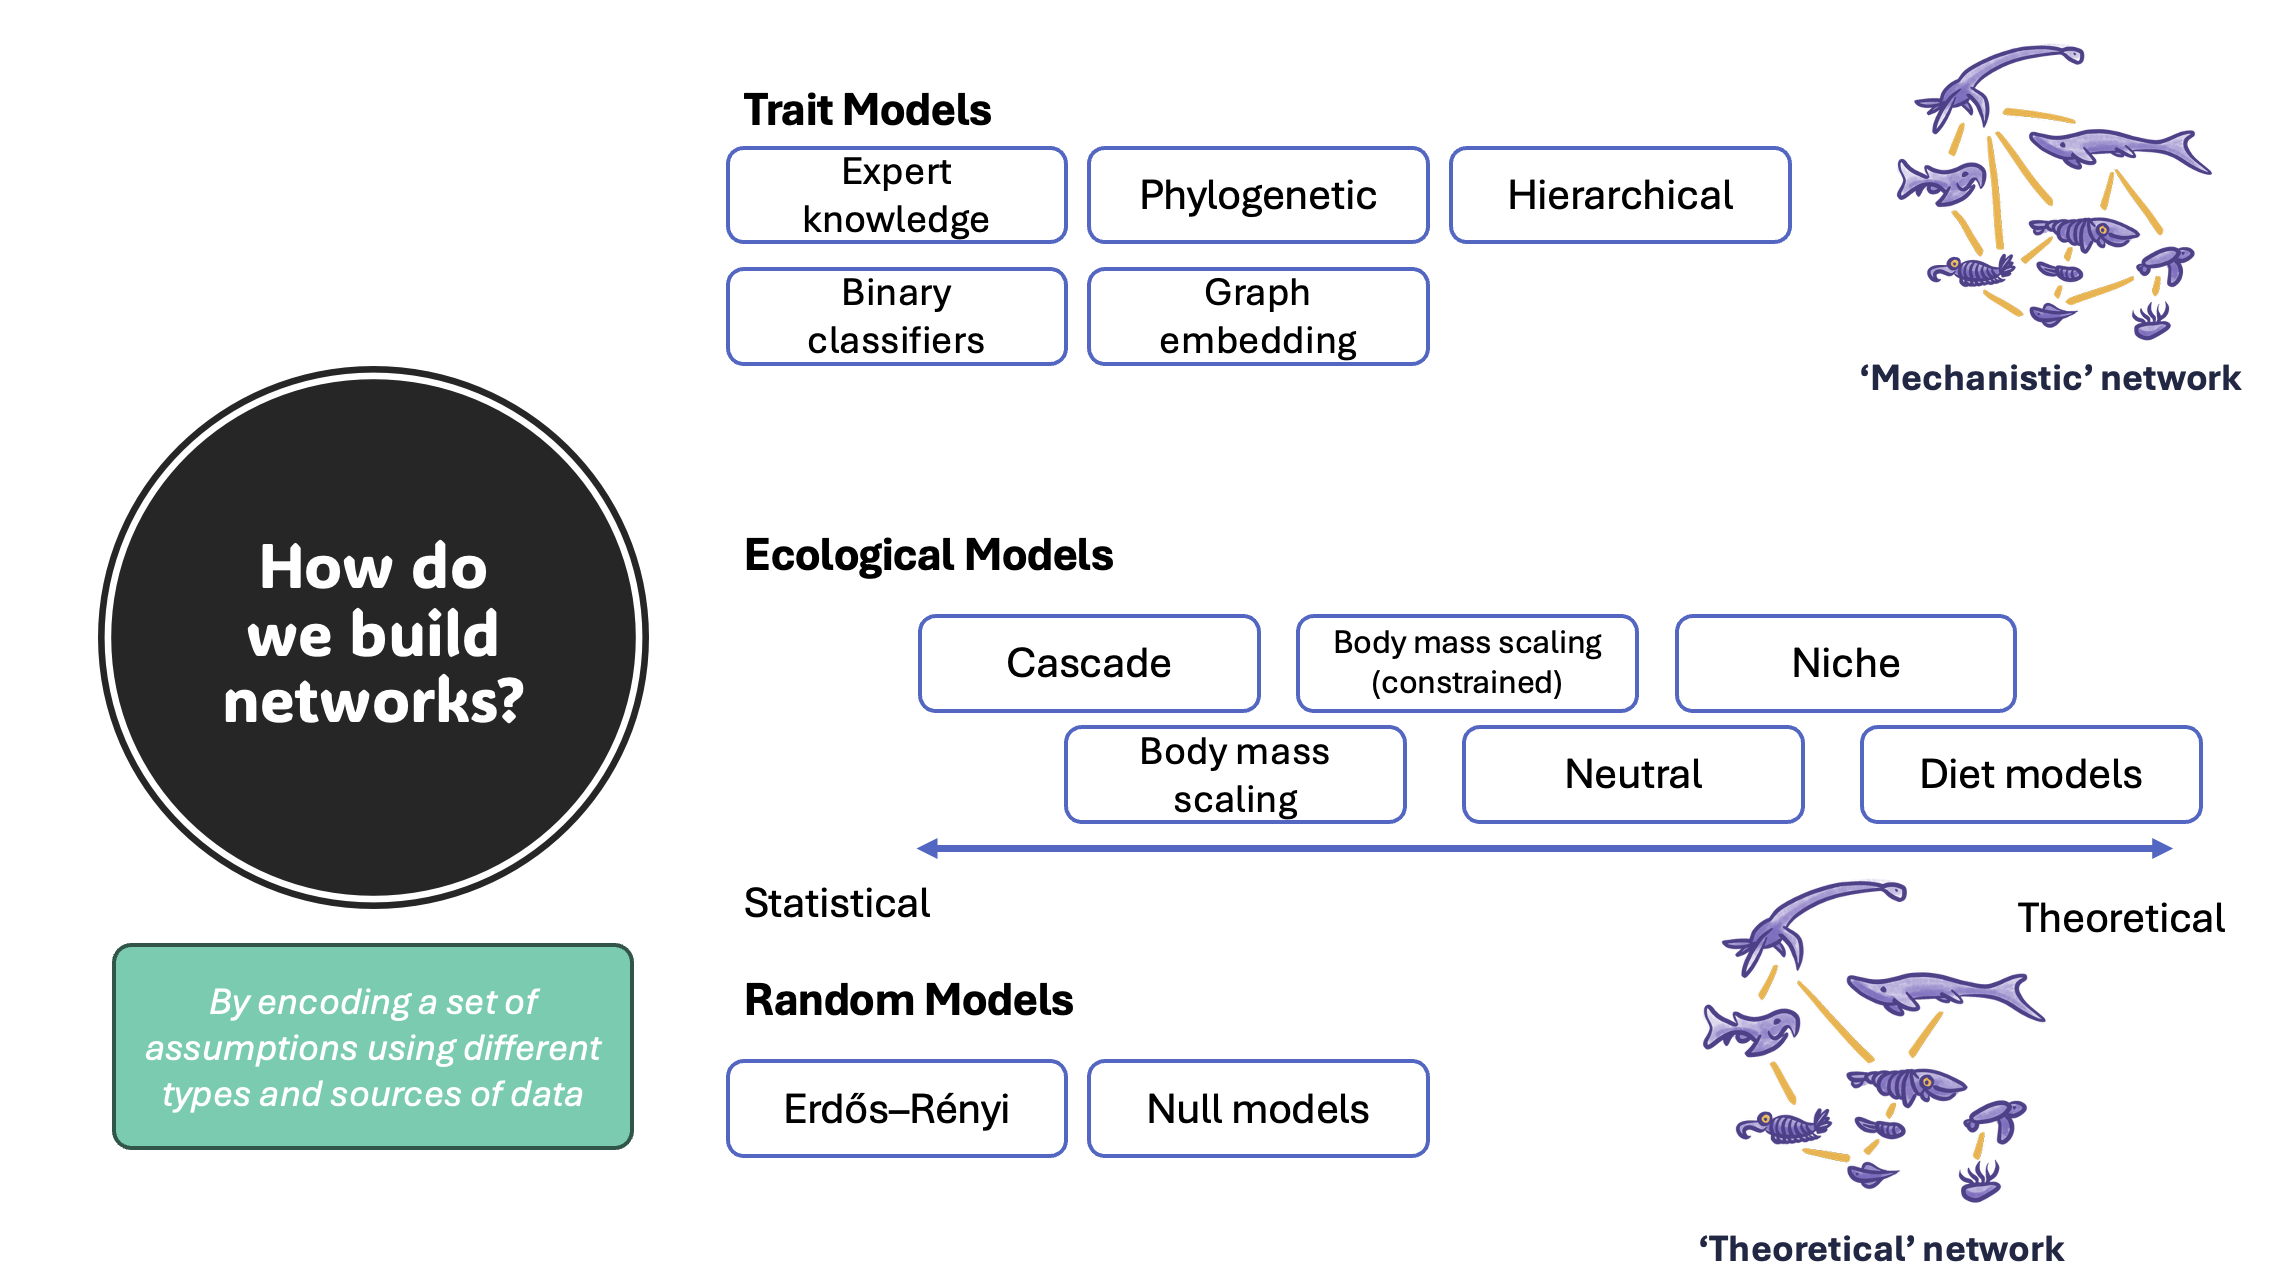
\includegraphics[keepaspectratio]{figures/model_fams.png}}

}

\caption{\label{fig-concept}This obviously needs work but a variation on
this to try and articulate the different approaches and broadly how they
may differ.}

\end{figure}%

Models that have specifically been developed in the paleo space tend to
be mechanistic models that focus on using a trait-based approach to
formalise feeding interactions (\emph{e.g.,} Shaw et al. (2024);
Roopnarine (2006)), are assembled by expert opinion (\emph{e.g.} Dunne
et al. (2014)) or make assumptions based on the evolutionary signals of
interactions (\emph{e.g.,} Fricke et al. (2022)). However, there is an
argument that the theoretical models that have been developed in
contemporary settings should hold even for paleo communities as we
expect the fundamental `currencies of life' to have remained constant -
\emph{e.g.,} the energetic constraints of foraging or foraging niches.
Along with constructing different Additionally there are models that
allow one to construct structurally sound networks that require very
little input data. These are methods that are amenable to the data
constraints that are prevalent in paleo communities in terms of both the
completeness of fossil records as well as how the deeper in time we move
the further away we might be moving from contemporary analogs.

Not all contemporary models may actually be suitable for paleo contexts
as the assumptions that they make (or the data that they require) may
actually introduce uncertainty/errors into the resulting network
rendering them of little use. Similarly not all paleo methods will be
suitable for all paleo communities. As a simple example the framework
developed by Fricke et al. (2022) uses phylogenetic relatedness as a way
to infer interactions of Pleistocene mammals by looking at how their
extant relatives interact. Although this approach is ecologically sound
(phylogenetic relatedness is also used in other approaches \emph{e.g.,}
Strydom et al. (2022)) there is also an argument that the further back
in evolutionary time we go (and the greater the phylogenetic distance
between extant and extinct communities become) there is more uncertainty
introduced by the phylogenetic tree than what is introduced by assuming
that interactions will be phylogenetically conserved.

\section{Challenges specific to building paleo
networks}\label{challenges-specific-to-building-paleo-networks}

Although there has been a push for the development of tools and methods
that allow us to predict species interactions and networks they will not
all be suitable for the prediction of paleo communities. This is
primarily due to limitations that we are faced with in terms of the
information that can be inferred from the fossil record (such as species
traits, abundances, and assemblages), which is needed as input data for
the different models. The limited information available from the fossil
record is compounded by the incomplete and biased preservation of
species {[}REF{]}, which part of a species is preserved (part vs whole),
the ambiguity of the `true' community composition {[}were communities
conserved \emph{in situ} or were they there owing to geological
processes?; REF{]}, as well as the availability/accessibility of
different rock layers (and thus the completeness of data we might have
for a specific era in time). Additionally there is an increasing degree
of `fuzziness' around the ecology and life histories of species the
further one moves back in geological time {[}REF{]}. This is not to say
that because we have imperfect data we should not be attempting to
construct paleo food webs but rather that we need to be aware of what
the uncertainties are and how these might impact the assumptions that we
need to make when constructing a network (as well as how this will
intersect with the intended end use of the network). This will allow us
to best identify an approach that minimises the assumption and potential
uncertainties within the data while still constructing a suitable
network. This includes thinking about both assumptions you are making
about the actual data \emph{e.g.,} trying to extrapolate body size from
fossil data but also assumptions across time \emph{e.g.,} assuming
modern trait-feeding modes are the same or that assumptions about
network structure will hold across deep time.

\subsection{Approaches to food web
prediction}\label{approaches-to-food-web-prediction}

Here we present six different models (Table~\ref{tbl-models}) that can
be used to construct food webs for both this specific community but are
also broadly suited to paleo network prediction. These models span all
facets of the network representation space (metaweb, realised, and
structural network) and are suitable for an array of different paleo
communities as the data requirements are `paleo friendly'.

\begin{longtable}[]{@{}
  >{\raggedright\arraybackslash}p{(\linewidth - 10\tabcolsep) * \real{0.1667}}
  >{\raggedright\arraybackslash}p{(\linewidth - 10\tabcolsep) * \real{0.1667}}
  >{\raggedright\arraybackslash}p{(\linewidth - 10\tabcolsep) * \real{0.1667}}
  >{\raggedright\arraybackslash}p{(\linewidth - 10\tabcolsep) * \real{0.1667}}
  >{\raggedright\arraybackslash}p{(\linewidth - 10\tabcolsep) * \real{0.1667}}
  >{\raggedright\arraybackslash}p{(\linewidth - 10\tabcolsep) * \real{0.1667}}@{}}
\caption{A summary of the different families of tools that can be used
to generate paleo food webs.}\label{tbl-models}\tabularnewline
\toprule\noalign{}
\begin{minipage}[b]{\linewidth}\raggedright
Model family
\end{minipage} & \begin{minipage}[b]{\linewidth}\raggedright
Assumptions
\end{minipage} & \begin{minipage}[b]{\linewidth}\raggedright
Data needs
\end{minipage} & \begin{minipage}[b]{\linewidth}\raggedright
`Limitation'
\end{minipage} & \begin{minipage}[b]{\linewidth}\raggedright
Network type
\end{minipage} & \begin{minipage}[b]{\linewidth}\raggedright
Key reference
\end{minipage} \\
\midrule\noalign{}
\endfirsthead
\toprule\noalign{}
\begin{minipage}[b]{\linewidth}\raggedright
Model family
\end{minipage} & \begin{minipage}[b]{\linewidth}\raggedright
Assumptions
\end{minipage} & \begin{minipage}[b]{\linewidth}\raggedright
Data needs
\end{minipage} & \begin{minipage}[b]{\linewidth}\raggedright
`Limitation'
\end{minipage} & \begin{minipage}[b]{\linewidth}\raggedright
Network type
\end{minipage} & \begin{minipage}[b]{\linewidth}\raggedright
Key reference
\end{minipage} \\
\midrule\noalign{}
\endhead
\bottomrule\noalign{}
\endlastfoot
random & Links are randomly distributed within a network & richness,
number of links & parameter assumptions, species agnostic & structural
network & Erdős \& Rényi (1959) \\
niche & Networks are interval, species can be ordered on a `niche axis'
& richness, connectance & parameter assumptions, species agnostic &
structural network & Williams \& Martinez (2008) \\
allometric diet breadth model (ADBM) & Interactions are determined by
energetic costs (foraging ecology) & body mass, biomass (abundance) &
does not account for forbidden links in terms of trait compatibility,
assumptions on body size and biomass (abundance) from fossil data &
theoretical network & Petchey et al. (2008) \\
l-matrix & Interactions inferred using allometric rules (ratio of body
sizes between predator and prey), with links being constrained by a
Ricker function & body mass, number of producer species & does not
account for forbidden links in terms of trait compatibility, assumptions
on body size from fossil data, assumptions as to the number of producer
species & theoretical network & Schneider et al. (2016) \\
paleo food web inference model (PFIM) & Interactions can be inferred by
a mechanistic framework/relationships & feeding traits for taxa,
mechanistic feeding rules & Assumption made as to the feeding
mechanisms, need to elucidate traits from models (although this is a way
smaller issue) & mechanistic web & Shaw et al. (2024) \\
body size ratio model & Interactions inferred using allometric rules
(ratio of body sizes between predator and prey). :ogit of the linking
probability used to further constrain links to an `optimal size range'
for prey. & body mass & does not account for forbidden links in terms of
evolutionary compatibility, assumptions on body size from fossil data &
theoretical network & Rohr et al. (2010) \\
\end{longtable}

\section{Case study: Toarcian mass extinction
event}\label{case-study-toarcian-mass-extinction-event}

\subsection{Dataset overview}\label{dataset-overview}

\subsubsection{Species occurrence}\label{species-occurrence}

Here we use the fossil occurrence data over an interval extends from the
upper Pliensbachian (\textasciitilde185 Ma) to the upper Toarcian
(\textasciitilde175 Ma) of the Cleveland Basin (see Dunhill et al., 2024
for a more comprehensive overview). The data set consists of a subset of
four broad time periods (pre-extinction, post-extinction, early
recovery, and late recovery). The assemblages are treated as communities
of interacting organisms. Something about the total number of taxa as
well as numbers per a time period? Probbaly also make a comment that
this is a `deep time' community we are looking at.

\subsubsection{Defining modes of life
(traits)}\label{defining-modes-of-life-traits}

We used the modes of life (traits) as identified in Dunhill et al.
(2024), who defined four traits: motility (fast, slow, facultative,
non-motile), tiering (pelagic, erect, surficial, semi-infaunal, shallow
infaunal, deep infaunal), feeding (predator, suspension feeder, deposit
feeder, mining, grazer), and size: gigantic (\textgreater500 mm), very
large (\textgreater300--500 mm), large (\textgreater100--300 mm), medium
(\textgreater50--100 mm), small (\textgreater10--50 mm), tiny (≤10 mm),
for each fossil species based on the ecological traits defined in the
Bambach ecospace model (Bambach et al., 2007).

\subsubsection{Constructing networks}\label{constructing-networks}

For each paleo community (time bin) we constructed \textbf{100} networks
for each model (so 6 * 100) networks. These networks were `simplified'
to removed any disconnected species. In total 2400 networks were
constructed. When a quantitative measure of body size is needed (ADBM,
bodymassratio, lmatrix) we drew a body mass for each species from a
uniform distribution. The ranges were defined by the different size
classes as discussed in insert cross ref to correct subsection here
\emph{e.g.,} a species classed as `very large' would have a body mass
drawn from \(U(300, 500)\). This was repeated for each run in order to
add variation to the networks constructed, however the same body sizes
were kept consistent for the relevant models (adbm, bodymassratio,
l-matrix) \emph{i.e.,} an ADBM and bodymassratio network from the same
rep number would have used the same bodysizes. The PFIM networks were
downsampled (see relevant section is S1). For both the random and niche
model the desired connectance was randomly selected between the range
0.07 - 0.15 for each repetition but kep consistent for both models. For
each network we calculated the properties listed in
Table~\ref{tbl-properties}

\subsection{Models capture different network structure but in unexpected
ways}\label{models-capture-different-network-structure-but-in-unexpected-ways}

Why is structure important and what can it tell us? Broadly when we talk
about quantifying the structure of a network we are interesting in
capturing some aspect of how the links are distributed between nodes, or
alternatively about properties of the nodes (specifically in terms of
the number of links coming in to (prey) or out of (predators) the node).
What are some things we can learn/infer from network structure: energy
flows and fluxes {[}REF{]}, propagation of stress {[}REF{]}, roles of
species in the community {[}REF, think trophic levels{]}. Some closing
statement about how thus there are different facets of network structure
and the value of understanding generally how different models differ in
terms of the structure that they recover - link to
Table~\ref{tbl-properties} maybe.

In terms of wanting to asses and compare across the different models it
is beneficial to approach this task by thinking about the different
aspects of the network as well as interactions that are being predicted
by the different models. It is perhaps beneficial to think of these
across different `scales' of organisation within the network, namely
macro (the entire network), meso (smaller interacting units within the
network), and micro (species-level attributes). Although there are a
myriad of possible ways to `measure' and analyse ecological networks
(Delmas et al., 2018) we do still lack a clear set of guidelines for
assessing how well models recover network structure (Allesina et al.,
2008) and it is beneficial to use a small subset of metrics that can
clearly be tied to broader aspects of network function or capturing a
ecological process.

Here we used a Multivariate Analysis Of Variance (MANOVA) as it is able
to capture model differences based on the combined information of the
multiple structural network measures. Model defined as
\texttt{network\ structure\ values\ \textasciitilde{}\ model\ +\ time\ period}
and Linear Discriminant Analysis (LDA) to determine if different models
produced networks with differing structure. \textbf{Need to report the
relevant effect of time in driving observed differences}

\begin{longtable}[]{@{}
  >{\raggedright\arraybackslash}p{(\linewidth - 6\tabcolsep) * \real{0.2466}}
  >{\raggedright\arraybackslash}p{(\linewidth - 6\tabcolsep) * \real{0.2603}}
  >{\raggedright\arraybackslash}p{(\linewidth - 6\tabcolsep) * \real{0.2466}}
  >{\raggedright\arraybackslash}p{(\linewidth - 6\tabcolsep) * \real{0.2466}}@{}}
\caption{An informative caption about the different network
properties}\label{tbl-properties}\tabularnewline
\toprule\noalign{}
\begin{minipage}[b]{\linewidth}\raggedright
Label
\end{minipage} & \begin{minipage}[b]{\linewidth}\raggedright
Definition
\end{minipage} & \begin{minipage}[b]{\linewidth}\raggedright
Scale
\end{minipage} & \begin{minipage}[b]{\linewidth}\raggedright
Reference (for maths), can make footnotes probs
\end{minipage} \\
\midrule\noalign{}
\endfirsthead
\toprule\noalign{}
\begin{minipage}[b]{\linewidth}\raggedright
Label
\end{minipage} & \begin{minipage}[b]{\linewidth}\raggedright
Definition
\end{minipage} & \begin{minipage}[b]{\linewidth}\raggedright
Scale
\end{minipage} & \begin{minipage}[b]{\linewidth}\raggedright
Reference (for maths), can make footnotes probs
\end{minipage} \\
\midrule\noalign{}
\endhead
\bottomrule\noalign{}
\endlastfoot
Connectance & \(L/S^2\), where \(S\) is the number of species and \(L\)
the number of links & Macro & \\
GenSD & Normalized standard deviation of generality of a species
standardized by \(L/S\) & Micro & Williams \& Martinez (2000) \\
LinkSD & Normalized standard deviation of links (number of consumers
plus resources per taxon) & Micro & \\
Richness & Number of nodes in the network & Macro & \\
TL & Prey-weighted trophic level averaged across taxa & Macro & Williams
\& Martinez (2004) \\
VulSD & Normalized standard deviation of vulnerability of a species
standardized by \(L/S\) & Micro & Williams \& Martinez (2000) \\
Diameter & Diameter can also be measured as the average of the distances
between each pair of nodes in the network & Macro & Delmas et al.
(2018) \\
\(\rho\) & Spectral radius is a a conceptual analog to nestedness (and
more appropriate for unipartite networks). It is defined as the absolute
value of the largest real part of the eigenvalues of the
\emph{undirected} adjacency matrix & Macro & Staniczenko et al.
(2013) \\
Complexity & SVD complexity of a network, defined as the Pielou entropy
of its singular values & Macro & Strydom et al. (2021a) \\
S1 & Number of linear chains & Meso & Milo et al. (2002); Stouffer et
al. (2007) \\
S2 & Number of omnivory motifs & Meso & Milo et al. (2002); Stouffer et
al. (2007) \\
S4 & Number of apparent competition motifs & Meso & Milo et al. (2002);
Stouffer et al. (2007) \\
S5 & Number of direct competition motifs & Meso & Milo et al. (2002);
Stouffer et al. (2007) \\
\end{longtable}

\subsubsection{Macro network properties}\label{macro-network-properties}

\textbf{Connectance} (Martinez, 1992) has been shown to be the feature
of networks that underpin a series of other properties and function
(Strydom et al., 2021b) and so it is perhaps the most important
structural attribute for a model to be able to retrieve correctly.
Additionally we consider the \textbf{complexity} of networks by
calculating their SVD entropy (this gives us an estimate of the physical
as opposed to behavioural complexity of networks; Strydom et al.
(2021a)), we could also look at the rank/rank deficiency of networks
which (theoretically) represents the number fo unique interaction
strategies in the network (Strydom et al., 2021a), which may be
specifically interesting in terms of looking at pre and post extinction
but also as a way to unpack `functional redundancy' that some models may
introduce.

\subsubsection{Meso network properties}\label{meso-network-properties}

Motifs represent smaller subset of interactions between three species,
and are argued to capture dynamics that are likely to be ecologically
relevant (Milo et al., 2002; Stouffer et al., 2007). Here we
specifically look at the number of \textbf{linear chains},
\textbf{omnivory}, \textbf{apparent competition}, and \textbf{direct
competition} motifs. In the broader context the ability of a model in
being able to capture these smaller motifs will inform as to its
suitability of use understanding the more dynamic component of network
ecology.

\subsubsection{Micro network properties}\label{micro-network-properties}

The number of interactions established (\textbf{generality}) or received
(\textbf{vulnerability}) by each species (Schoener, 1989), are (broadly)
indicative of consumer-resource relationships and diet breadth of
species {[}ref{]}. Although this is usually determined at the species
level the standard deviation of the generality and vulnerability of
species is often used when benchmarking predicted networks (Petchey et
al., 2008; \emph{e.g.,} Williams \& Martinez, 2008).

The \textbf{specificity} of species in a network is measured as a
function of the proportion of resources they effectively use (Poisot et
al., 2012)

\begin{figure}

\centering{

\pandocbounded{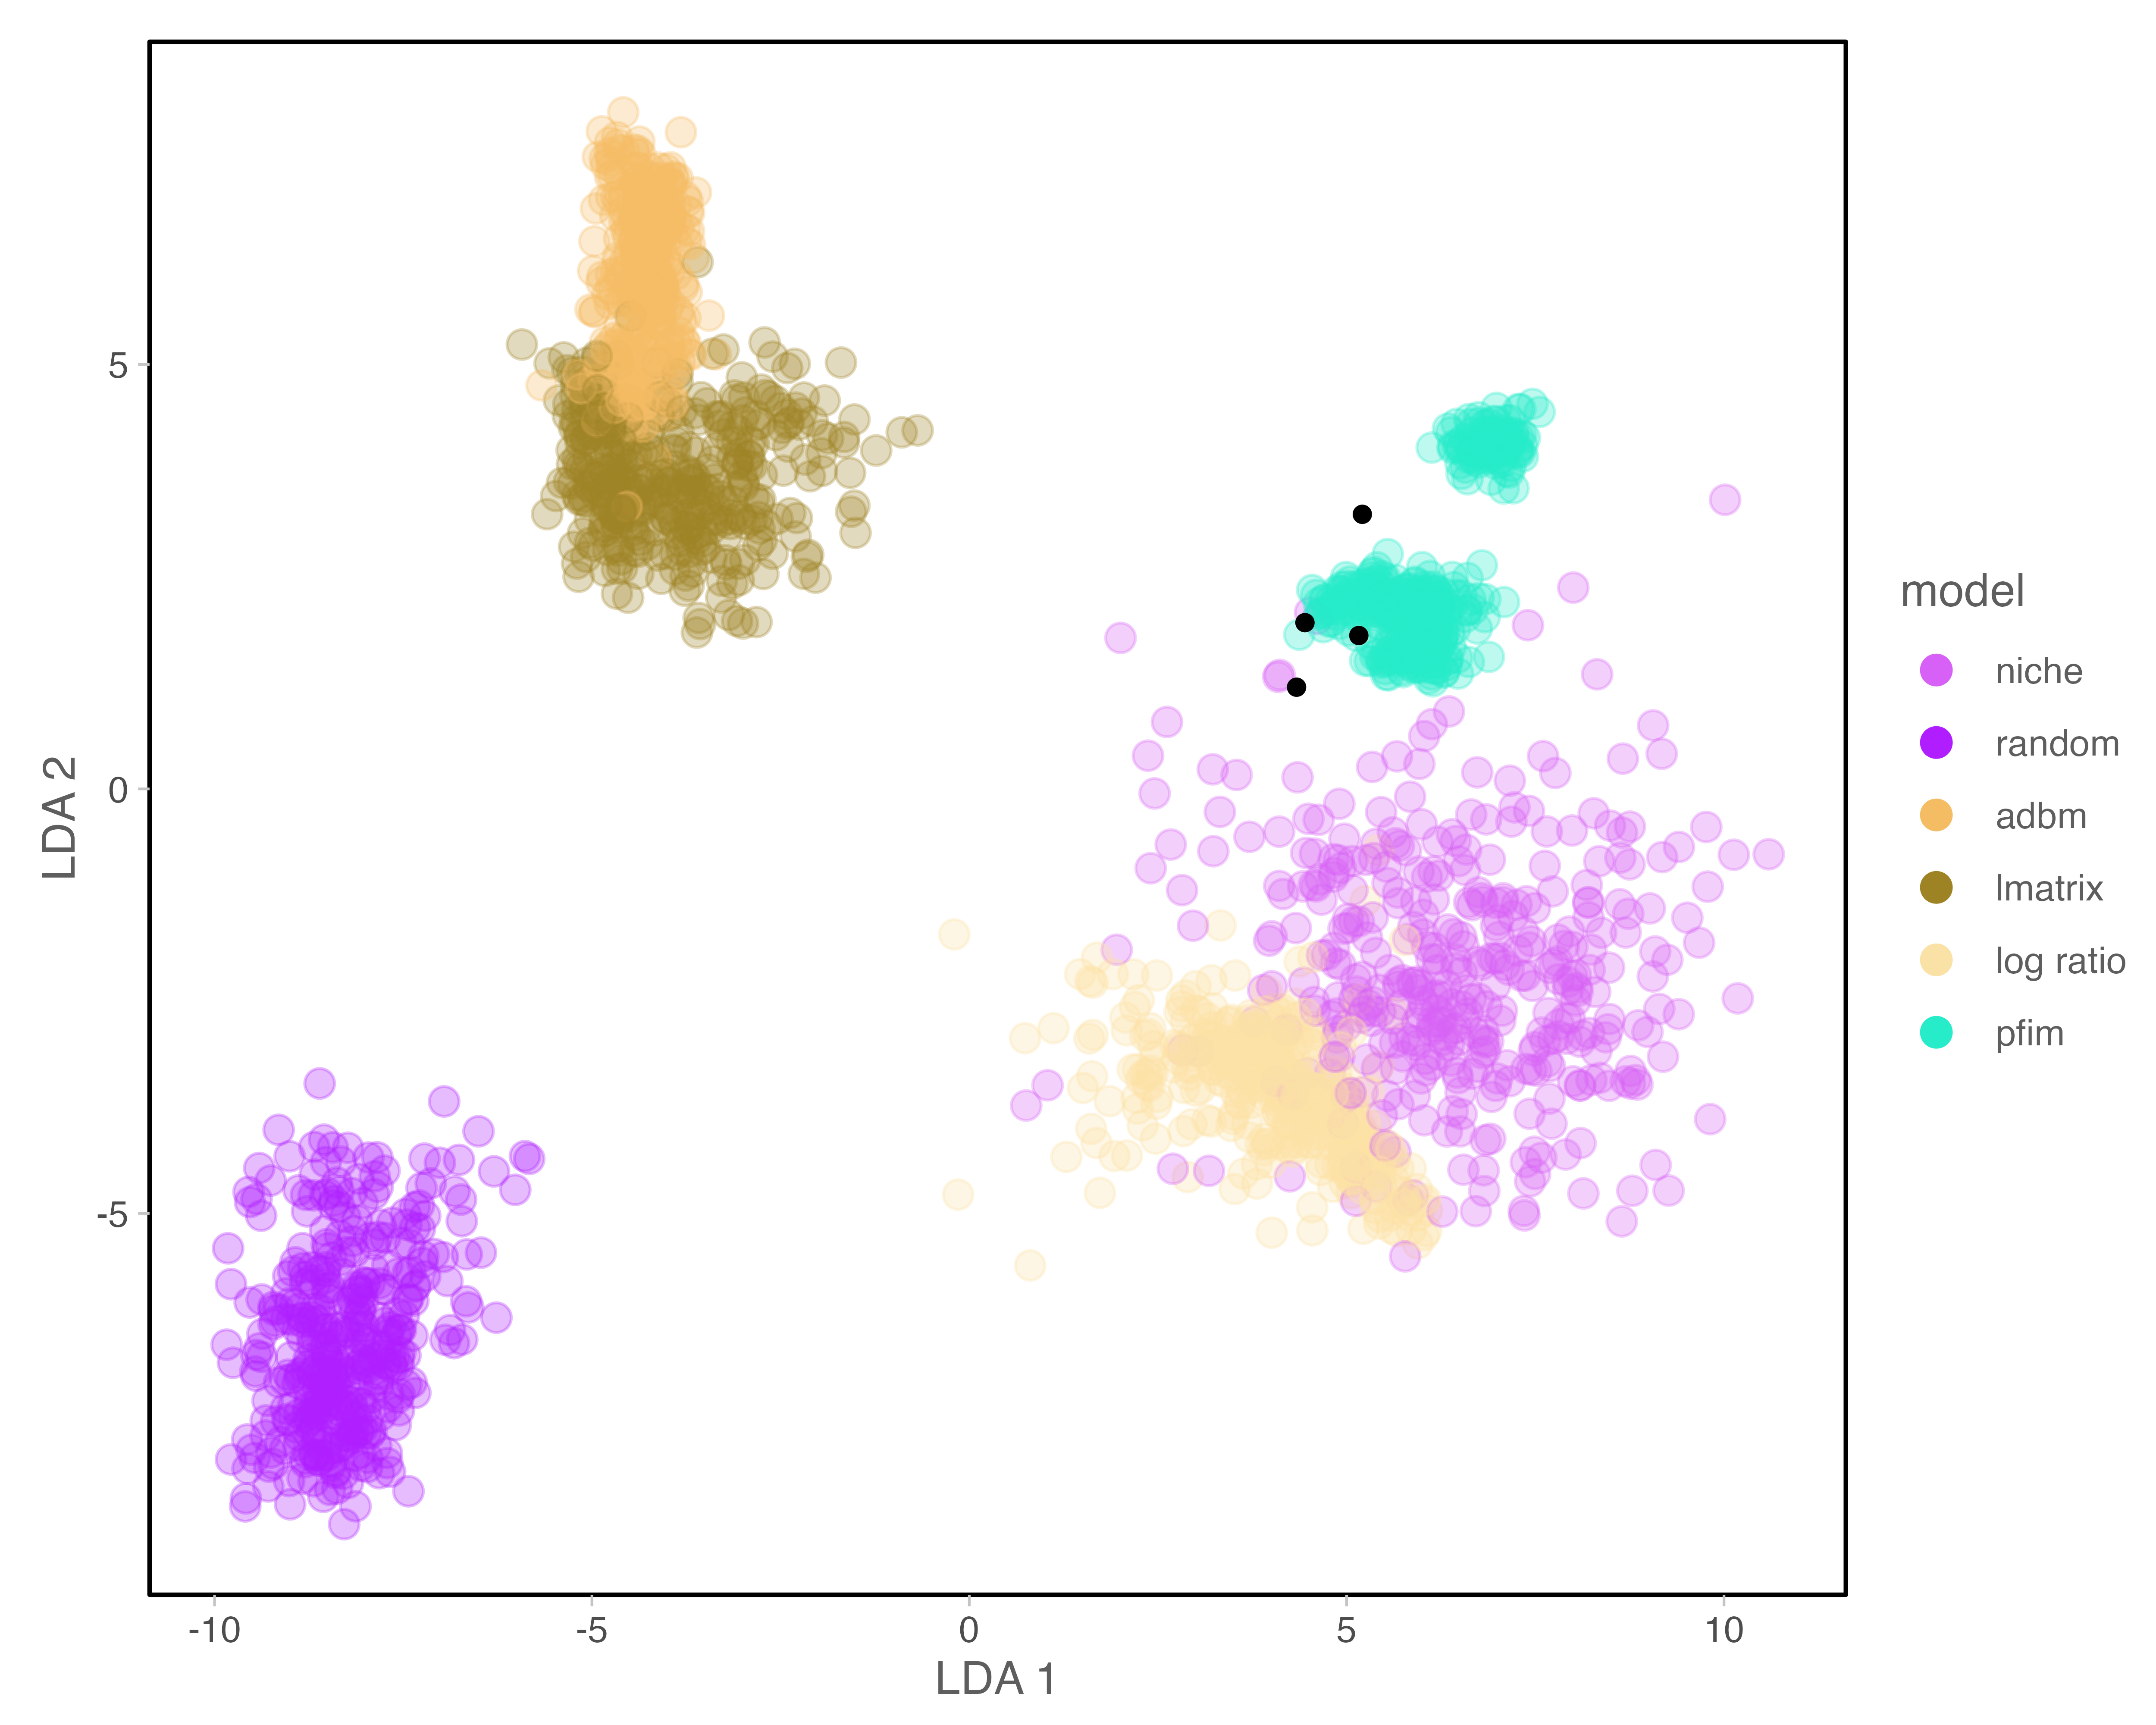
\includegraphics[keepaspectratio]{figures/MANOVA_lda.png}}

}

\caption{\label{fig-structure}stuff\ldots{}}

\end{figure}%

What is perhaps the most striking result in Figure~\ref{fig-structure}
is that although there are clear structural differences between the
different models the differences are not distinct between the broader
model families but rather that there is a degree of overlap between them
(specifically the log ratio, PFIM, and niche models). Although the log
ratio and niche models are classified as different families they are
built on similar ecological background and theory and so it is perhaps
not surprising that these networks capture a similar structure (the same
holds for the ADBM and l-matrix models). The fact that the random model
occupies a completely different space is unsurprising as it has clearly
been shown that networks are non-random in nature {[}REF{]} and so we
expect random models to be constructing ecologically illogical networks.
What is perhaps the most interesting result is that the PFIM model
constructs networks that are very similar to those that are rooted in
niche-based processes despite the model being more mechanistic in
nature. Not sure how to articulate but this is cool because the is
\emph{something} in network structure constraints that is straddling the
trait-niche space of ecology - but also see my next point about it being
`correct' is still up for debate

Although it is not possible to confidently identify the models that are
predicting the \emph{`correct'} network structure the fact that a models
from different families are able to recover similar structures is
reassuring as it suggests that it might be possible to substitute one
model for another if the input data is insufficient.

\begin{quote}
\textbf{TODO} Is it sound to try and unpack the `pairwise differences'
between the different structural metrics as well (or some) as this will
allow us to say e.g.~Niche and PFIM might recover the same connectance
but differ in vulnerability.
\end{quote}

\subsection{Some networks don't share any interactions and some share a
lot}\label{some-networks-dont-share-any-interactions-and-some-share-a-lot}

In addition to wanting to measure network structure researchers may also
be interested in understanding aspects about the diets and predators of
\emph{specific} species in a community. In this instance the interest
should be in understanding how the pairwise links predicted between
species pairs differ between models. Here we look ath the interaction
turnover (Poisot et al., 2012) both within and between the different
models. This can be thought of as the equivalent of species \(\beta\)
turnover and tells us which interactions are `conserved' (shared) across
the networks but only between species pairs that are shared -
\emph{i.e.,} this turnover is only driven by interaction and not species
turnover. Here we only compared networks that we constructed for the
same period (as our interest is only in between model differences) and
excluded the random and niche networks from consideration as these two
models are essentially species agnostic.

\begin{figure}

\centering{

\pandocbounded{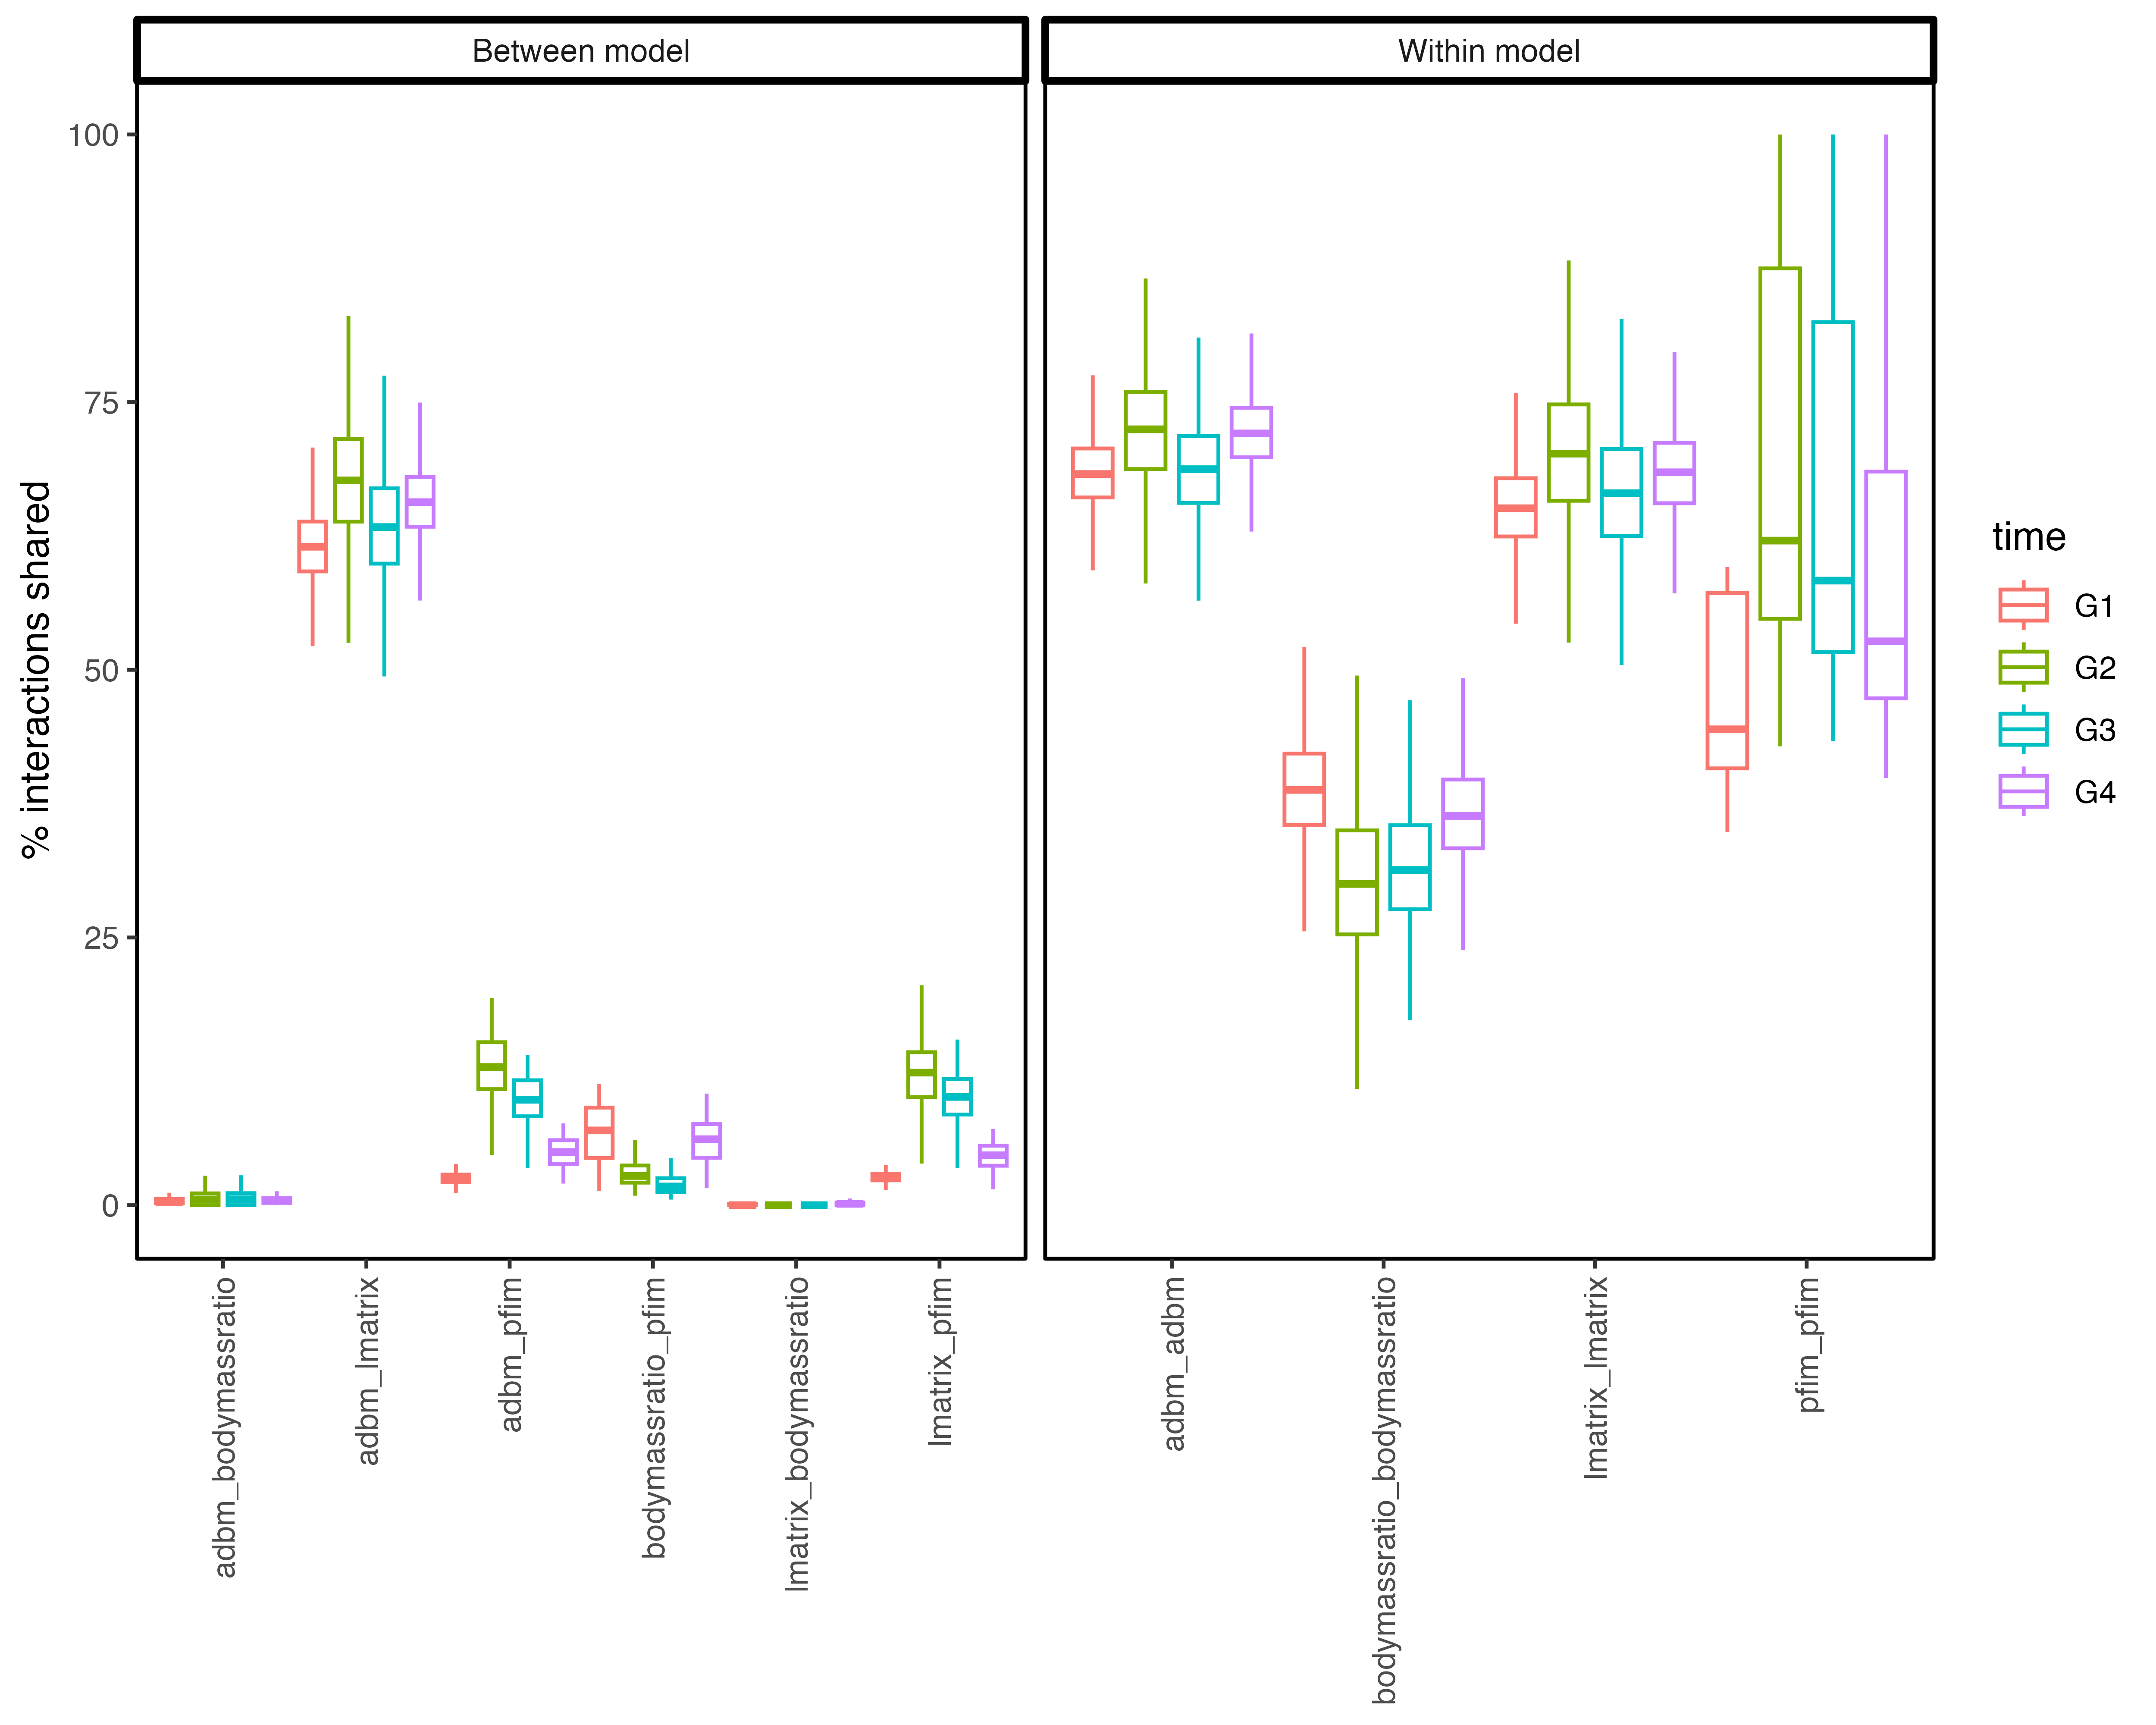
\includegraphics[keepaspectratio]{figures/beta_div.png}}

}

\caption{\label{fig-beta_div}stuff\ldots{} \% interaction shared is
calculated as number shared interactions / ((number interactions left -
shared interactions) + (number interactions right - shared interactions)
+ shared interactions). Additionally niche and random models are
excluded as it is illogical since both of these models are fundamentally
species agnostic}

\end{figure}%

In Figure~\ref{fig-beta_div} it is clear that some models share a large
percentage of interactions \emph{e.g.,} between ADBM and l-matrix
networks and others share nothing \emph{e.g.,} ADBM and PFIM networks.
This result is unsurprising as the mechanisms that determine
interactions in ADBM and l-matrix (a single trait (bodysize) + some
ecological theory) is very different from the PFIM model that makes
assumptions on a trait-based hierarchy.

The key takeaway that this needs to lead into is thinking about diet
related questions and the model that is best suited to get you there. It
makes sense to contextualise this in the feasible vs realised
interaction spectrum - specifically that from a `philosophical' basis if
you are asking questions about possible diets of species then it makes
sense to use models that fall firmly in the `feasible' space
\emph{e.g.,} PFIM model or even something like the Fricke et al. (2022)
model. How these results support that is that we can see the ADBM and
PFIM are recovering (almost) totally different pairwise links.

\subsection{Model choice changes the
narrative}\label{model-choice-changes-the-narrative}

\paragraph{Simulating Extinctions}\label{simulating-extinctions}

Extinctions were simulated using different plausible mechanisms based on
both species traits (size, motility), their position within the network
(generality, vulnerability), as well as randomly. Each network was
subjected to \textbf{50} extinction runs for each extinction mechanisms.
The extinctions themselves were cascading in nature meaning that after
the target species was removed all species that no longer had any prey
were also deemed as extinct (secondary extinction), checking for
secondary extinctions was then repeated until there were no longer any
species without prey. This represents one extinction event and only then
would the proceeding target species be removed from the network and
cascading extinctions assessed again. Note that for extinction
simulations which use the network position of a species to determine
extinction order we follow the protocol from Curtsdotter et al. (2011)
and reassess the vulnerability/generality of each species after each
extinction event to `redetermine' the extinction order.

As we are using Dunhill et al. (2024) as a case study we followed their
appraoch when simulating extinctions as well as assessing which
extinction mechanism results in a simulated network that most closely
matches the real post extinciton network. Extinction simulations were
only run on the pre extinction networks whereby species were removed
until they reached the `target richness', which is the richness of the
post extinction community. In order to determine which extinction
mechnism creates a network most similar to the post extinction network
we used the (get full name of score) TSS (Gupta et al., 2022) to assess
how different the pairwise interactions are between `simulated' and
`real' post extinction communities as well as looking at the absolute
differences in network structure metrics.

\begin{quote}
\textbf{TODO} not sure if we also want to unpack/showcase robustness
\(R_{50}\) (Jonsson et al., 2015)
\end{quote}

\begin{figure}

\centering{

\pandocbounded{\includegraphics[keepaspectratio]{figures/dunhill_comp.png}}

}

\caption{\label{fig-dunhill}stuff\ldots{} Recreation of the figure from
Dunhill 2024. Note not 100\% sold on the TSS and absolute mean
calculations\ldots{}}

\end{figure}%

\subsubsection{Trends over time}\label{trends-over-time}

\begin{quote}
\textbf{TODO} Not sure statistically speaking what the best way to
unpack this is\ldots{} 2-way ANOVA/ANCOVA explanation is valuable? There
are intercept differences (\emph{e.g.,} baseline average values are
different; are the rankings among all three response variables the
same?) and there are shape differences/similarities (\emph{e.g.,} motifs
are all the same shape but Co and Gen show some among model differences
in pattern.)
\end{quote}

Visual take-away seems to suggest that we see that the values
(intercepts) of the different summary statistics are different but
(broadly) they are capturing the same trends. This might suggest that
although we observe differences in structure
(Figure~\ref{fig-structure}) the general patterns still remain the same.
This is good news because it means that at least the models that we have
used here tend to tell us the same general story - which is worth
contextualising in the space of `right' vs `wrong' and as long as we are
not fixated on the point value but rather on understanding the trends.

\subsubsection{Inferred extinction
drivers}\label{inferred-extinction-drivers}

Points of discussion one will be to point to the mean absolute distance
and how generally the ADBM/l-matrix do really badly - high mean absolute
value. And this maybe makes sense though because of how we specify
extinction mechanisms (trait-based) and so it sets the body-size models
are not `talking' the same language. In terms of the TSS scores - not
sure how we should unpack it. Individually by model family to see which
model agrees with which appraoch and see if different mechanisms come
out stronger? \textbf{TODO} still need to sanity check the TSS
anyway\ldots{}

\section{Discussion (need a catchier
heading)}\label{discussion-need-a-catchier-heading}

I want this section to be more about contextualising model choice within
the bigger research question discussion - i.e.~mapping question and
model choice more tightly\ldots{}

Points to discuss:

\begin{itemize}
\tightlist
\item
  Guidlines - as a box? Can we give something concrete??
\item
  How to we synthesise these results? As in should we give clear
  directives ot is it enough to do a bit more handwaving and have the
  bigger message be that model choice matters?
\end{itemize}

\section*{References}\label{references}
\addcontentsline{toc}{section}{References}

\phantomsection\label{refs}
\begin{CSLReferences}{1}{0}
\bibitem[\citeproctext]{ref-allesina2008}
Allesina, S., Alonso, D., \& Pascual, M. (2008). A general model for
food web structure. \emph{Science}, \emph{320}(5876), 658--661.
\url{https://doi.org/10.1126/science.1156269}

\bibitem[\citeproctext]{ref-bambach2007}
Bambach, R. K., Bush, A. M., \& Erwin, D. H. (2007). Autecology and the
Filling of Ecospace: Key Metazoan Radiations. \emph{Palaeontology},
\emph{50}(1), 1--22.
\url{https://doi.org/10.1111/j.1475-4983.2006.00611.x}

\bibitem[\citeproctext]{ref-curtsdotter2011}
Curtsdotter, A., Binzer, A., Brose, U., De Castro, F., Ebenman, B.,
Eklöf, A., Riede, J. O., Thierry, A., \& Rall, B. C. (2011). Robustness
to secondary extinctions: Comparing trait-based sequential deletions in
static and dynamic food webs. \emph{Basic and Applied Ecology},
\emph{12}(7), 571--580. \url{https://doi.org/10.1016/j.baae.2011.09.008}

\bibitem[\citeproctext]{ref-delmas2018}
Delmas, E., Besson, M., Brice, M.-H., Burkle, L. A., Dalla Riva, G. V.,
Fortin, M.-J., Gravel, D., Guimarães, P. R., Hembry, D. H., Newman, E.
A., Olesen, J. M., Pires, M. M., Yeakel, J. D., \& Poisot, T. (2018).
Analysing ecological networks of species interactions. \emph{Biological
Reviews}, 112540. \url{https://doi.org/10.1111/brv.12433}

\bibitem[\citeproctext]{ref-dillon2022}
Dillon, E. M., Pier, J. Q., Smith, J. A., Raja, N. B., Dimitrijević, D.,
Austin, E. L., Cybulski, J. D., De Entrambasaguas, J., Durham, S. R.,
Grether, C. M., Haldar, H. S., Kocáková, K., Lin, C.-H., Mazzini, I.,
Mychajliw, A. M., Ollendorf, A. L., Pimiento, C., Regalado Fernández, O.
R., Smith, I. E., \& Dietl, G. P. (2022). What is conservation
paleobiology? Tracking 20 years of research and development.
\emph{Frontiers in Ecology and Evolution}, \emph{10}.
\url{https://doi.org/10.3389/fevo.2022.1031483}

\bibitem[\citeproctext]{ref-dunhill2024}
Dunhill, A. M., Zarzyczny, K., Shaw, J. O., Atkinson, J. W., Little, C.
T. S., \& Beckerman, A. P. (2024). Extinction cascades, community
collapse, and recovery across a Mesozoic hyperthermal event.
\emph{Nature Communications}, \emph{15}(1), 8599.
\url{https://doi.org/10.1038/s41467-024-53000-2}

\bibitem[\citeproctext]{ref-dunne2014}
Dunne, J. A., Labandeira, C. C., \& Williams, R. J. (2014). Highly
resolved early eocene food webs show development of modern trophic
structure after the end-cretaceous extinction. \emph{Proceedings of the
Royal Society B: Biological Sciences}, \emph{281}(1782), 20133280.
\url{https://doi.org/10.1098/rspb.2013.3280}

\bibitem[\citeproctext]{ref-erdos1959}
Erdős, P., \& Rényi, A. (1959). On random graphs. i. \emph{Publicationes
Mathematicae Debrecen}, \emph{6}(3-4), 290--297.
\url{https://doi.org/10.5486/pmd.1959.6.3-4.12}

\bibitem[\citeproctext]{ref-fricke2022}
Fricke, E. C., Hsieh, C., Middleton, O., Gorczynski, D., Cappello, C.
D., Sanisidro, O., Rowan, J., Svenning, J.-C., \& Beaudrot, L. (2022).
Collapse of terrestrial mammal food webs since the Late Pleistocene.
\emph{Science}, \emph{377}(6609), 1008--1011.
\url{https://doi.org/10.1126/science.abn4012}

\bibitem[\citeproctext]{ref-gauzens2025}
Gauzens, B., Thouvenot, L., Srivastava, D. S., Kratina, P., Romero, G.
Q., Berti, E., O'Gorman, E. J., González, A. L., Dézerald, O.,
Eisenhauer, N., Pires, M., Ryser, R., Farjalla, V. F., Rogy, P., Brose,
U., Petermann, J. S., Geslin, B., \& Hines, J. (2025). Tailoring
interaction network types to answer different ecological questions.
\emph{Nature Reviews Biodiversity}, 1--10.
\url{https://doi.org/10.1038/s44358-025-00056-7}

\bibitem[\citeproctext]{ref-gupta2022}
Gupta, A., Furrer, R., \& Petchey, O. L. (2022). Simultaneously
estimating food web connectance and structure with uncertainty.
\emph{Ecology and Evolution}, \emph{12}(3), e8643.
\url{https://doi.org/10.1002/ece3.8643}

\bibitem[\citeproctext]{ref-hao2025}
Hao, X., Holyoak, M., Zhang, Z., \& Yan, C. (2025). Global Projection of
Terrestrial Vertebrate Food Webs Under Future Climate and Land-Use
Changes. \emph{Global Change Biology}, \emph{31}(2), e70061.
\url{https://doi.org/10.1111/gcb.70061}

\bibitem[\citeproctext]{ref-jonsson2015}
Jonsson, T., Berg, S., Pimenov, A., Palmer, C., \& Emmerson, M. (2015).
The reliability of R50 as a measure of vulnerability of food webs to
sequential species deletions. \emph{Oikos}, \emph{124}(4), 446--457.
\url{https://doi.org/10.1111/oik.01588}

\bibitem[\citeproctext]{ref-jordano2016}
Jordano, P. (2016). Chasing Ecological Interactions. \emph{PLOS
Biology}, \emph{14}(9), e1002559.
\url{https://doi.org/10.1371/journal.pbio.1002559}

\bibitem[\citeproctext]{ref-kiessling2019}
Kiessling, W., Raja, N. B., Roden, V. J., Turvey, S. T., \& Saupe, E. E.
(2019). Addressing priority questions of conservation science with
palaeontological data. \emph{Philosophical Transactions of the Royal
Society B: Biological Sciences}, \emph{374}(1788), 20190222.
\url{https://doi.org/10.1098/rstb.2019.0222}

\bibitem[\citeproctext]{ref-martinez1992}
Martinez, N. D. (1992). Constant connectance in community food webs.
\emph{The American Naturalist}, \emph{139}(6), 1208--1218.
\url{http://www.jstor.org/stable/2462337}

\bibitem[\citeproctext]{ref-milo2002}
Milo, R., Shen-Orr, S., Itzkovitz, S., Kashtan, N., Chklovskii, D., \&
Alon, U. (2002). Network motifs: Simple building blocks of complex
networks. \emph{Science}, \emph{298}(5594), 824--827.
\url{https://doi.org/10.1126/science.298.5594.824}

\bibitem[\citeproctext]{ref-morales-castilla2015}
Morales-Castilla, I., Matias, M. G., Gravel, D., \& Araújo, M. B.
(2015). Inferring biotic interactions from proxies. \emph{Trends in
Ecology \& Evolution}, \emph{30}(6), 347--356.
\url{https://doi.org/10.1016/j.tree.2015.03.014}

\bibitem[\citeproctext]{ref-petchey2008}
Petchey, O. L., Beckerman, A. P., Riede, J. O., \& Warren, P. H. (2008).
Size, foraging, and food web structure. \emph{Proceedings of the
National Academy of Sciences}, \emph{105}(11), 4191--4196.
\url{https://doi.org/10.1073/pnas.0710672105}

\bibitem[\citeproctext]{ref-pichler2023}
Pichler, M., \& Hartig, F. (2023). Machine learning and deep
learning{\textemdash}A review for ecologists. \emph{Methods in Ecology
and Evolution}, \emph{14}(4), 994--1016.
\url{https://doi.org/10.1111/2041-210X.14061}

\bibitem[\citeproctext]{ref-poisot2012}
Poisot, T., Canard, E., Mouquet, N., \& Hochberg, M. E. (2012). A
comparative study of ecological specialization estimators. \emph{Methods
in Ecology and Evolution}, \emph{3}(3), 537--544.
\url{https://doi.org/10.1111/j.2041-210x.2011.00174.x}

\bibitem[\citeproctext]{ref-rohr2010}
Rohr, R., Scherer, H., Kehrli, P., Mazza, C., \& Bersier, L.-F. (2010).
Modeling food webs: Exploring unexplained structure using latent traits.
\emph{The American Naturalist}, \emph{176}(2), 170--177.
\url{https://doi.org/10.1086/653667}

\bibitem[\citeproctext]{ref-roopnarine2006}
Roopnarine, P. D. (2006). Extinction cascades and catastrophe in ancient
food webs. \emph{Paleobiology}, \emph{32}(1), 1--19.
\url{https://www.jstor.org/stable/4096814}

\bibitem[\citeproctext]{ref-schneider2016}
Schneider, F. D., Brose, U., Rall, B. C., \& Guill, C. (2016). Animal
diversity and ecosystem functioning in dynamic food webs. \emph{Nature
Communications}, \emph{7}(1), 12718.
\url{https://doi.org/10.1038/ncomms12718}

\bibitem[\citeproctext]{ref-schoener1989}
Schoener, T. W. (1989). Food Webs From the Small to the Large: The
Robert H. MacArthur Award Lecture. \emph{Ecology}, \emph{70}(6),
1559--1589. \url{https://doi.org/10.2307/1938088}

\bibitem[\citeproctext]{ref-shaw2024}
Shaw, J. O., Dunhill, A. M., Beckerman, A. P., Dunne, J. A., \& Hull, P.
M. (2024). \emph{A framework for reconstructing ancient food webs using
functional trait data} (p. 2024.01.30.578036). bioRxiv.
\url{https://doi.org/10.1101/2024.01.30.578036}

\bibitem[\citeproctext]{ref-staniczenko2013}
Staniczenko, P. P. A., Kopp, J. C., \& Allesina, S. (2013). The ghost of
nestedness in ecological networks. \emph{Nature Communications},
\emph{4}(1), 1391. \url{https://doi.org/10.1038/ncomms2422}

\bibitem[\citeproctext]{ref-stouffer2007}
Stouffer, D. B., Camacho, J., Jiang, W., \& Nunes Amaral, L. A. (2007).
Evidence for the existence of a robust pattern of prey selection in food
webs. \emph{Proceedings of the Royal Society B: Biological Sciences},
\emph{274}(1621), 1931--1940.
\url{https://doi.org/10.1098/rspb.2007.0571}

\bibitem[\citeproctext]{ref-strydom2022}
Strydom, T., Bouskila, S., Banville, F., Barros, C., Caron, D., Farrell,
M. J., Fortin, M.-J., Hemming, V., Mercier, B., Pollock, L. J., Runghen,
R., Dalla Riva, G. V., \& Poisot, T. (2022). Food web reconstruction
through phylogenetic transfer of low-rank network representation.
\emph{Methods in Ecology and Evolution}, \emph{13}(12).
\url{https://doi.org/10.1111/2041-210X.13835}

\bibitem[\citeproctext]{ref-strydom2021b}
Strydom, T., Catchen, M. D., Banville, F., Caron, D., Dansereau, G.,
Desjardins-Proulx, P., Forero-Muñoz, N. R., Higino, G., Mercier, B.,
Gonzalez, A., Gravel, D., Pollock, L., \& Poisot, T. (2021b). A roadmap
towards predicting species interaction networks (across space and time).
\emph{Philosophical Transactions of the Royal Society B: Biological
Sciences}, \emph{376}(1837), 20210063.
\url{https://doi.org/10.1098/rstb.2021.0063}

\bibitem[\citeproctext]{ref-strydom2021}
Strydom, T., Catchen, M. D., Banville, F., Caron, D., Dansereau, G.,
Desjardins-Proulx, P., Forero-Muñoz, N. R., Higino, G., Mercier, B.,
Gonzalez, A., Gravel, D., Pollock, L., \& Poisot, T. (2021a). A roadmap
towards predicting species interaction networks (across space and time).
\emph{Philosophical Transactions of the Royal Society B: Biological
Sciences}, \emph{376}(1837), 20210063.
\url{https://doi.org/10.1098/rstb.2021.0063}

\bibitem[\citeproctext]{ref-thuiller2024}
Thuiller, W., Calderón-Sanou, I., Chalmandrier, L., Gaüzère, P.,
O'Connor, L. M. J., Ohlmann, M., Poggiato, G., \& Münkemüller, T.
(2024). Navigating the integration of biotic interactions in
biogeography. \emph{Journal of Biogeography}, \emph{51}(4), 550--559.
\url{https://doi.org/10.1111/jbi.14734}

\bibitem[\citeproctext]{ref-williams2000}
Williams, R. J., \& Martinez, N. D. (2000). Simple rules yield complex
food webs. \emph{Nature}, \emph{404}(6774), 180--183.
\url{https://doi.org/10.1038/35004572}

\bibitem[\citeproctext]{ref-williams2004}
Williams, R. J., \& Martinez, N. D. (2004). Stabilization of chaotic and
non-permanent food-web dynamics. \emph{The European Physical Journal B -
Condensed Matter}, \emph{38}(2), 297--303.
\url{https://doi.org/10.1140/epjb/e2004-00122-1}

\bibitem[\citeproctext]{ref-williams2008}
Williams, R. J., \& Martinez, N. D. (2008). Success and its limits among
structural models of complex food webs. \emph{The Journal of Animal
Ecology}, \emph{77}(3), 512--519.
\url{https://doi.org/10.1111/j.1365-2656.2008.01362.x}

\bibitem[\citeproctext]{ref-yeakel2014}
Yeakel, J. D., Pires, M. M., Rudolf, L., Dominy, N. J., Koch, P. L.,
Guimarães, P. R., \& Gross, T. (2014). Collapse of an ecological network
in ancient egypt. \emph{PNAS}, \emph{111}(40), 14472--14477.
\url{https://doi.org/10.1073/pnas.1408471111}

\end{CSLReferences}





\end{document}
